\subsection{Effectiveness of Training Data Synthesis}
\label{subsec:data_effectiveness}

% \begin{figure}[t]
    \centering
    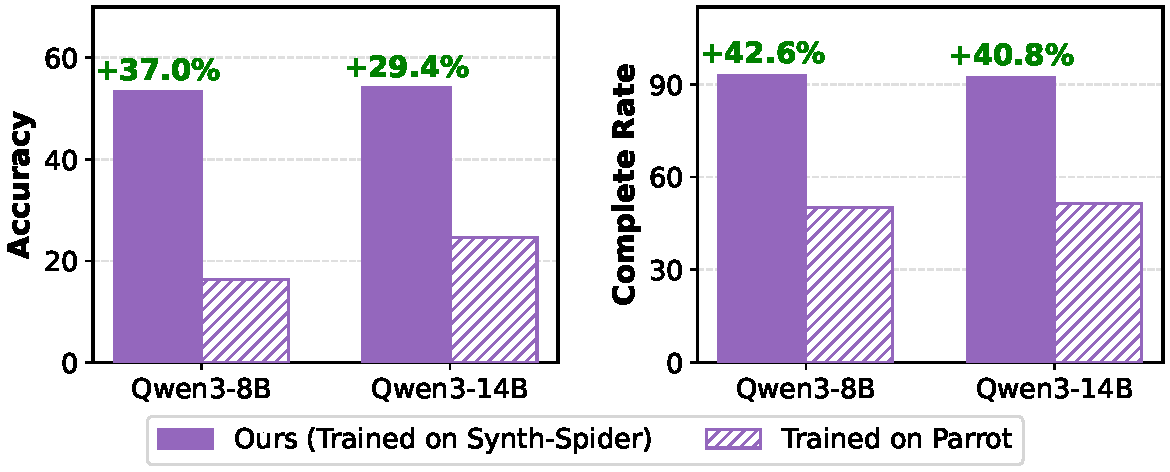
\includegraphics[width=0.99\columnwidth]{plots/plot/trained_on_spider_and_parrot_eval_bird.pdf}
    \vspace{-0.5em} 
    \caption{Evaluation results on Synth-Bird (Dev) of models trained on Synth-Spider (Train) and Parrot (Train).}
    \label{fig:trained_on_spider_and_parrot_eval_bird}
    \vspace{-0.5em}
\end{figure}
% \begin{figure}[t]
    \centering
    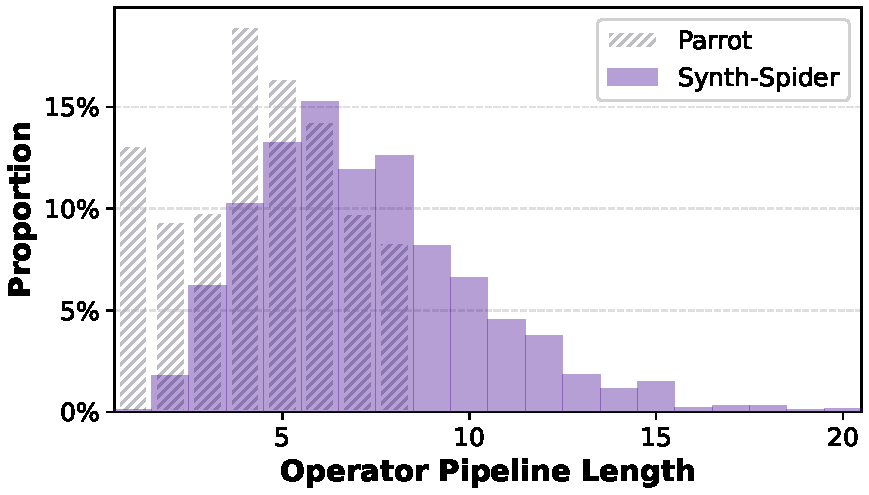
\includegraphics[width=0.95\columnwidth]{plots/plot/op_len_distribution.pdf}
    \vspace{-1em} 
    \caption{Operator Pipeline Length Distribution.}
    \label{fig:op_len_distribution}
    \vspace{-0.5em}
    % \vspace{-1em}
\end{figure}
\begin{figure}[t]
    \centering
    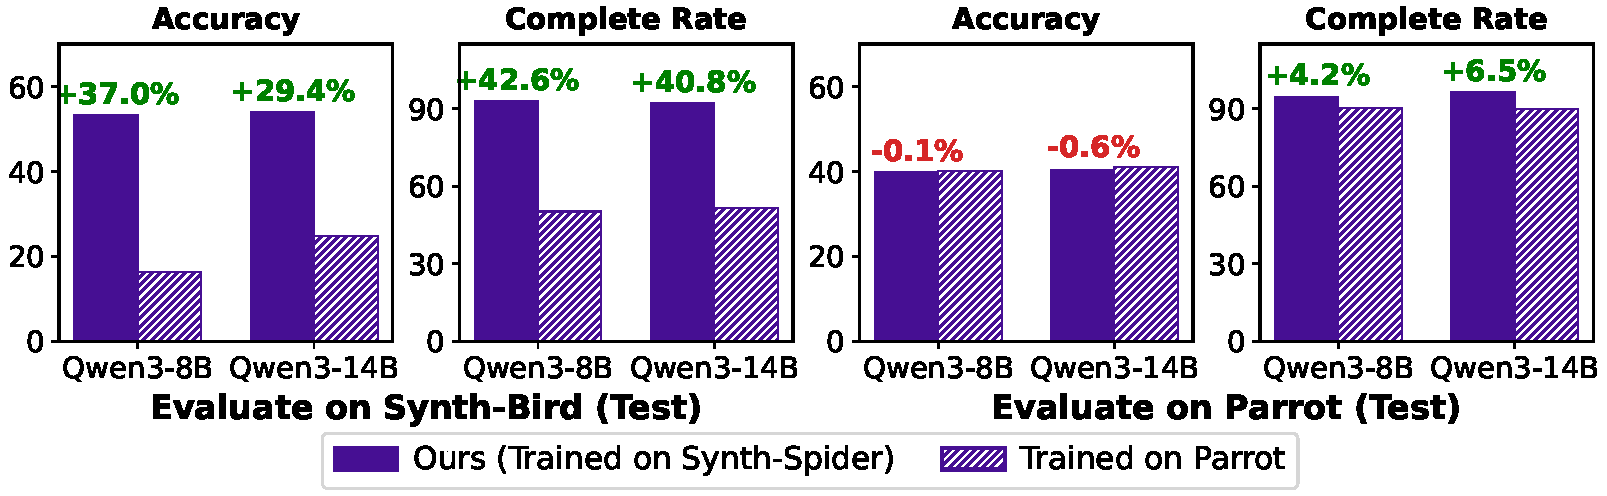
\includegraphics[width=1.01\columnwidth]{plots/plot/trained_on_spider_and_parrot.pdf}
    \vspace{-2em} 
    \caption{Evaluation results of models trained on Synth-Spider (Train) and Parrot (Train).}
    \label{\labelprefix fig:trained_on_spider_and_parrot}
    \vspace{-1em}
\end{figure}

\stitle{Exp-\expnum\label{exp:data_effectiveness}: Effectiveness of Synthesized Training Data.}
We evaluate whether models trained on our synthesized Synth-Spider training set generalize better than those trained on the public Parrot training set. 
% Both models are evaluated on the Synth-Bird Test set.
We first evaluate these two models on Synth-Bird (Test) under the out-of-domain setting. As illustrated on the left part of Figure~\ref{fig:trained_on_spider_and_parrot}, training on Synth-Spider yields much higher performance: accuracy increases by 37.0 and 29.4 points on Qwen3-8B and Qwen3-14B over Parrot. 
% Completion rate shows even larger gains, with increases of 42.6 and 40.8 respectively.
To further highlight the effectiveness of synthesized data, we adopt a more challenging setting. We evaluate on Parrot (Test) of models trained on Synth-Spider (totally out-of-domain setting) and models trained on Parrot (in-domain setting). As illustrated on the right of Figure~\ref{fig:trained_on_spider_and_parrot}. Our synthesized data is even competitive under such challenging experiment setting. Models trained on Synth-Spider achieve comparable accuracy to the model trained on Parrot (40.44 vs. 40.99 on Qwen3-8B). 

% These consistent gains show that our synthesized training data provide more effective supervision for agentic training than existing public data.
% The stronger generalization of Synth-Spider lies in the diversity and complexity of synthesized DP pipelines.
% First, as shown in Table~\ref{tbl:datasets}, Synth-Spider has more long-horizon operator and provides broader operator coverage than Parrot. Second, Synth-Spider has more diverse operator combination. We have conducted a fine-grained analysis of operator compositional diversity between these two datasets. Synth-Spider produces 496 unique bigrams and 2,875 unique trigrams, compared to Parrot’s 189 and 758 respectively. Moreover, Synth-Spider’s top-5 and top-10 bigram concentration ratios are also lower than Parrot’s (0.226 and 0.326 vs. 0.248 and 0.361), indicating that its operator distribution is less dominated by a few frequent patterns.
% In summary, the more diverse and complex pipelines in Synth-Spider promotes tree-based agentic reasoning during agentic training, in turn improving generalization capabilities to unseen data.


% To understand why Synth-Spider yields stronger generalization, we compare operator-pipeline length distributions of the two training datasets in Figure~\ref{fig:op_len_distribution}. Parrot samples cluster on shorter pipelines, while Synth-Spider consistently contains more medium- and long-horizon operator pipelines.
% This adds procedural complexity to promotes tree-based agentic reasoning during agentic training, in turn improving generalization capabilities to unseen data.

\begin{shaded}
\noindent \textbf{Finding \findingnum: 
Our synthetic training data provides effective supervision for agentic training, significantly improving the performance on unseen tasks.
%Our data synthesis strategy fosters robust planning, significantly improving task completion rates on unseen tasks without compromising accuracy.
}
\end{shaded}